%%%%%%%%%%%%%%%%%%%%%%%%%%%%%%%%%%%%%%%%%%%%%%%%%%%%%%%%%%%%%%%%%%%%%%%%%%%%%%%%
%           Capitulo 6: Descripcion del archivo de configuracion               %
%%%%%%%%%%%%%%%%%%%%%%%%%%%%%%%%%%%%%%%%%%%%%%%%%%%%%%%%%%%%%%%%%%%%%%%%%%%%%%%%

\chapter{Descripción del archivo de configuración}

Como se ha podido ver hasta ahora, el archivo de configuración definido por el usuario
juega un papel clave en el sistema. Es gracias a él que la mayoría de operaciones dentro
del sistema pueden ser automatizadas, como por ejemplo la generación de problemas, la
traducción de estados de observación a estados \texttt{PDDL}, la gestión de objetivos
y la traducción de planes. Por tanto, es importante conocerlo más a fondo. En las secciones
posteriores se describirá el proceso de creación del archivo de configuración, el formato
que tiene y su estructura mediante un ejemplo concreto, el cual facilitará su comprensión.

\section{Creación del archivo}

Como se comentó brevemente en el capítulo anterior, la creación del archivo de configuración
está semiautomatizada. Se tiene un \textit{script} que, dado un archivo que contiene el dominio
\texttt{PDDL} y el archivo de descripción del juego en formato \texttt{VGDL}, genera un archivo
de configuración plantilla para que el usuario lo pueda rellenar. Algunos de los campos de
ese archivo ya estarán rellenados, pero se deja total libertad al usuario para que los modifique.
También existen ciertos campos que son opcionales, aunque se concretará más cuáles son cuando
se describa la estructura del archivo.

\section{Formato del archivo de configuración}

El archivo de configuración está en formato \texttt{YAML} (\textit{YAML Ain't Markup Language}),
que es un lenguaje para la serialización de datos creado de forma que sea muy fácil de leer tanto
por humanos como por la máquina. Es esta legibilidad lo que hace que \texttt{YAML} sea ideal para
la creación de archivos de configuración, ya que de manera sencilla y clara se pueden establecer
los parámetros que configuran un sistema.

El lenguaje está formado por tipos básicos como cadenas de texto, enteros, números reales y valores
booleanos. También tiene tipos más avanzados, como listas y relaciones clave-valor.

\section{Estructura del archivo de configuración}

Para explicar la estructura del archivo vamos a partir de un archivo de configuración plantilla
generado para el juego \textit{Boulderdash}. A partir de este archivo plantilla se explicarán los campos
que lo forman y cómo se rellenarían. El juego como tal se explicará más detalladamente en capítulos
posteriores, pero la idea general es coger 9 de las gemas que hay en el mapa y salir del
nivel, esquivando a los enemigos (cangrejos y mariposas) y picando las rocas para despejar el camino.
El nivel de ejemplo que se va a utilizar se puede ver en la figura \ref{fig:boulderdash-example}.

\begin{figure}[H]
    \centering
    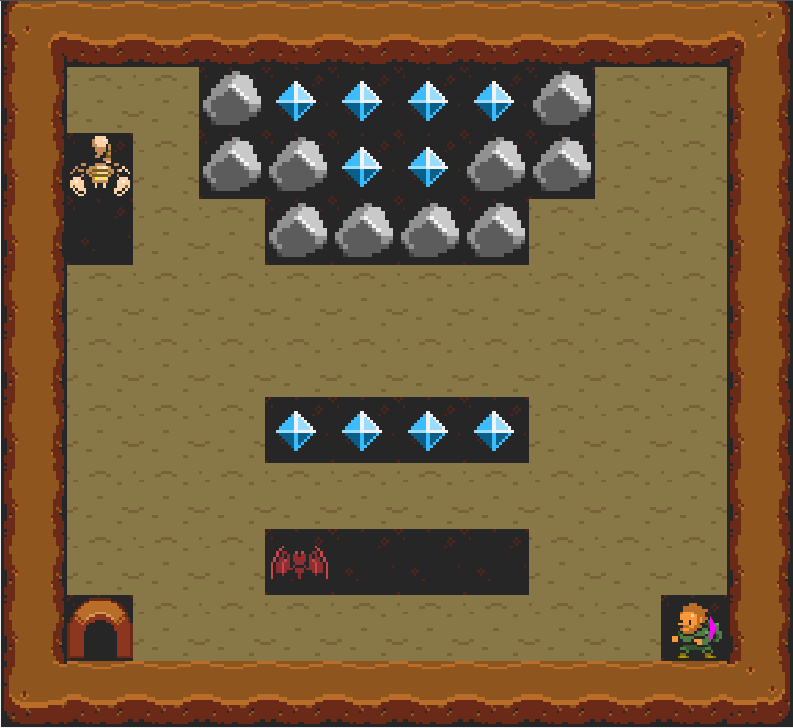
\includegraphics[scale=0.4]{img/CH06/boulderdash.png}
    \caption{Nivel de ejemplo del juego \textit{Boulderdash}.}
    \label{fig:boulderdash-example}
\end{figure}

\begin{lstlisting}[language=pddl,
    caption={Dominio \texttt{PDDL} del juego \textit{Boulderdash}.},
    label={lst:boulderdash},
    captionpos=b]
  (:types
    Bat Scorpion - Enemy
    Gem Player Boulder Enemy Exit - Locatable
    Cell
  )

  (:predicates
    (at ?l - Locatable ?c - Cell)
    (oriented-up ?p - Player)
    (oriented-down ?p - Player)
    (oriented-left ?p - Player)
    (oriented-right ?p - Player)
    (connected-up ?c1 ?c2 - Cell)
    (connected-down ?c1 ?c2 - Cell)
    (connected-left ?c1 ?c2 - Cell)
    (connected-right ?c1 ?c2 - Cell)
    (terrain-ground ?c - Cell)
    (terrain-wall ?c - Cell)
    (terrain-empty ?c - Cell)
    (got ?g - Gem)
    (exited-level)
    (occupied ?c - Cell)
  )

  (:action turn-up
    ... )

  (:action turn-down
    ... )

  (:action turn-left
    ... )

  (:action turn-right
    ... )

  (:action move-up
    ... )

  (:action move-down
    ... )

  (:action move-left
    ... )

  (:action move-right
    ... )
  
  (:action move-up-get-gem
    ... )

  (:action move-down-get-gem
    ... )

  (:action move-left-get-gem
    ... )

  (:action move-right-get-gem
    ... )

  (:action dig-up
    ... )

  (:action dig-down
    ... )

  (:action dig-left
    ... )

  (:action dig-right
    ... )

  (:action exit-level
    ... )
\end{lstlisting}

Es importante también conocer el dominio \texttt{PDDL} que se ha creado para el juego, el cual puede
verse de forma resumida en el listado \ref{lst:boulderdash} y se utilizará en la explicación que se
va a realizar. Se pueden ver los tipos que representan a los elementos del juego, los predicados y las acciones
que puede realizar, aunque éstas se muestran de forma simplificada (solo el nombre). A continuación se ofrece más
información sobre lo que representan los predicados:

\begin{itemize}[label=\textbullet]
    \item El predicado \texttt{(at ?l - Locatable ?c - Cell)}, que indica que un objeto determinado
    se encuentra en una determinada celda.
    \item Los predicados \texttt{(oriented-up ?p - Player)}, \texttt{(oriented-down ?p - Player)},
    \texttt{(oriented-left ?p - Player)} y \texttt{(oriented-right ?p - Player)}, los cuales expresan
    la orientación del jugador.
    \item Los predicados \texttt{(connected-up ?c1 ?c2 - Cell)}, \texttt{(connected-down ?c1 ?c2 - Cell)},
    \texttt{(connected-left ?c1 ?c2 - Cell)} y \texttt{(connected-right ?c1 ?c2 - Cell)}, los cuales sirven
    para representar las relaciones de conectividad entre las casillas. Por ejemplo, el primero de ellos indica
    que la celda \texttt{?c1} tiene por encima de ella a la casilla \texttt{?c2}. Algo similar sucede con el
    siguiente predicado, donde se indica que \texttt{?c2} estaría debajo de \texttt{?c1}. Y así con el resto
    de predicados, los cuales tienen una semántica igual a estos dos casos.
    \item Los predicados \texttt{(terrain-ground ?c - Cell)}, \texttt{(terrain-wall ?c - Cell)} y
    \texttt{(terrain-empty ?c - Cell)} indican el tipo de terreno de la celda (con tierra, muro o excavada,
    respectivamente).
    \item El predicado \texttt{(got ?g - Gem)} indica que se ha cogido la gema \texttt{?g}.
    \item El predicado \texttt{(exited-level)} indica que se ha salido el nivel una vez que se han cogido
    las gemas necesarias.
    \item El predicado \texttt{(occupied ?c - Cell)} indica que la celda está ocupada por una roca o un enemigo.
\end{itemize}

Por último, es importante comentar brevemente qué representa cada acción:

\begin{itemize}
    \item Las acciones \texttt{turn-up}, \texttt{turn-down}, \texttt{turn-left} y \texttt{turn-right}
    representan el giro que puede realizar el agente para cambiar su orientación a la que indique el nombre
    de la acción.
    \item Las acciones \texttt{move-up}, \texttt{move-down}, \texttt{move-left} y \texttt{move-right}
    implican el movimiento del agente de una casilla a otra que esté conectada con la primera, siempre y
    cuando el agente esté orientado de la forma correcta y exista una conexión entre las dos casillas.
    Por ejemplo, si se quiere mover hacia arriba (\texttt{move-up}), tendrá que estar orientado hacia arriba y
    tendrá que existir un predicado \texttt{(connected-up c1 c2)} que indique que existe la correspondiente
    conexión entre ambas celdas.
    \item Las acciones \texttt{move-up-get-gem}, \texttt{move-down-get-gem}, \texttt{move-left-get-gem}
    y \texttt{move-right-get-gem} son parecidas a las cuatro anteriores, solo que si hay una gema en
    la casilla destino, el agente la coge en el proceso.
    \item Las acciones \texttt{dig-up}, \texttt{dig-down}, \texttt{dig-left} y \texttt{dig-right} implican
    cavar en la dirección que indican. Para ello, el agente tiene que estar orientado previamente de forma
    correcta.
    \item La acción \texttt{exit-level} se lleva a cabo cuando el agente va a salir del nivel, una vez
    que ha cogido todas las gemas necesarias.
\end{itemize}

Una vez descritos el juego y el dominio \texttt{PDDL} que se ha creado para el juego, pasemos a comentar
la estructura del archivo de configuración. A continuación se ofrece el contenido de la plantilla que
se ha obtenido a la hora de ejecutar el \textit{script}:

\begin{lstlisting}[language=yaml]
domainFile: domains/boulderdash-domain.pddl
problemFile: problem.pddl
domainName: BoulderDash
cellVariable: null
avatarVariable: null
gameElementsCorrespondence:
  background:
  - null
  wall:
  - null
  sword:
  - null
  dirt:
  - null
  exitdoor:
  - null
  diamond:
  - null
  boulder:
  - null
  avatar:
  - null
  crab:
  - null
  butterfly:
  - null
variablesTypes:
  ?variable: Type
orientationCorrespondence:
  UP: null
  DOWN: null
  LEFT: null
  RIGHT: null
connections:
  UP: null
  DOWN: null
  LEFT: null
  RIGHT: null
actionsCorrespondence:
  TURN-UP: ACTION_UP
  TURN-DOWN: ACTION_DOWN
  TURN-LEFT: ACTION_LEFT
  TURN-RIGHT: ACTION_RIGHT
  MOVE-UP: ACTION_UP
  MOVE-DOWN: ACTION_DOWN
  MOVE-LEFT: ACTION_LEFT
  MOVE-RIGHT: ACTION_RIGHT
  MOVE-UP-GET-GEM: ACTION_UP
  MOVE-DOWN-GET-GEM: ACTION_DOWN
  MOVE-LEFT-GET-GEM: ACTION_LEFT
  MOVE-RIGHT-GET-GEM: ACTION_RIGHT
  DIG-UP: ACTION_UP
  DIG-DOWN: ACTION_DOWN
  DIG-LEFT: ACTION_LEFT
  DIG-RIGHT: ACTION_RIGHT
  EXIT-LEVEL: null
goals:
- goalPredicate: null
  priority: 0
  saveGoal: false
  removeReachedGoalsList:
  - null
\end{lstlisting}

Los campos que aparecen en el fichero son los siguientes:

\begin{enumerate}
    \item \texttt{domainFile}: Nombre del fichero de dominio \texttt{PDDL}. Este campo se genera
    automáticamente a partir de los parámetros utilizados a la hora de ejecutar el \textit{script}.
    
    \item \texttt{problemFile}: Nombre del fichero de problema de salida. Tiene como valor por defecto
    \texttt{problem.pddl}, pero el usuario puede darle el nombre que quiera.
    
    \item \texttt{domainName}: Nombre del dominio. Se genera automáticamente y se obtiene a partir del
    archivo de dominio \texttt{PDDL}.
    
    \item  \label{enum:cell} \texttt{cellVariable}: Variable que se utilizará para representar las celdas. Una
    variable viene precedida por el símbolo ``\texttt{?}'' y se le da el nombre que quiera el usuario. El uso del
    símbolo de interrogación es para que tenga cierta semejanza con la manera en la que se hacen las definiciones
    de variables en \texttt{PDDL}. Por ejemplo, en este caso se ha decidido que dicha variable sea la
    siguiente:
    
    \begin{lstlisting}[language=yaml]
cellVariable: ?c
    \end{lstlisting}
    
    Supongamos que hemos asociado el predicado \texttt{(at ?l - Locatable ?c - Cell)} del domino
    \texttt{PDDL} a una serie de elementos del juego. En este caso, la variable \texttt{?c} que se ha
    definido en el dominio se correspondería con la variable que hemos definido en el fichero de configuración,
    la cual es \texttt{?c}. Es importante destacar que no tienen por qué tener el mismo nombre. Por ejemplo,
    podríamos haberle puesto el nombre \texttt{?celda} en el archivo de configuración. Cuando el traductor se
    encuentre con alguno de los elementos a los que está asociado el predicado, sustituirá en este predicado la variable \texttt{?c} por su instancia correspondiente, la cual será \texttt{c\_x\_y}, donde \texttt{x} es la
    columna e \texttt{y} la fila donde se encuentra dicho elemento del juego.
    
    \item \texttt{avatarVariable}: Variable que se utilizará para representar al avatar/agente. Por
    ejemplo, en este caso se ha decidido que sea la siguiente:
    
    \begin{lstlisting}[language=yaml]
avatarVariable: ?p
    \end{lstlisting}
    
    Esta variable es especial, ya que cuando se encuentre dicha variable en alguno de los predicados asociados
    al avatar se va a sustituir simplemente por el nombre que le ha dado el usuario. Por ejemplo,
    en este caso se sustituiría por \texttt{p}. Se ha hecho de esta forma debido a que simplifica
    mucho la monitorización del plan, ya que tener una variable que constantemente cambia sus coordenadas
    $x,y$ solo induciría a errores.
    
    \item \texttt{gameElementsCorrespondence}: Este campo sirve para asociar una lista de predicados
    a cada observación (elemento) del juego, de forma que cuando el traductor de estados de observación
    se encuentre con dicha observación, generará los correspondientes predicados instanciando las variables
    de la misma forma que se describió en el punto \ref{enum:cell}, a excepción como se comentó en el
    punto anterior de las variables asociadas al jugador, las cuales se instancian de forma especial.
    Las observaciones se obtienen a partir del fichero que define el juego en formato \texttt{VGDL}, el
    cual recordemos que se pasa como parámetro a la hora de generar la plantilla del archivo de configuración.
    Una observación que aparece siempre es \texttt{background}, la cual representa una celda en la que no
    hay nada. Para este juego en concreto se han definido las siguientes correspondencias:
    
    \begin{lstlisting}[language=yaml]
gameElementsCorrespondence:
  background:
  - (terrain-empty ?c)
  wall:
  - (terrain-wall ?c)
  sword:
  - (terrain-empty ?c)
  dirt:
  - (terrain-ground ?c)
  exitdoor:
  - (at ?e ?c)
  - (terrain-empty ?c)
  diamond:
  - (at ?g ?c)
  - (terrain-empty ?c)
  - (occupied ?c)
  boulder:
  - (at ?boulder ?c)
  - (terrain-empty ?c)
  - (occupied ?c)
  avatar:
  - (at ?p ?c)
  - (terrain-empty ?c)
  crab:
  - (at ?s ?c)
  - (terrain-empty ?c)
  - (occupied ?c)
  butterfly:
  - (at ?b ?c)
  - (terrain-empty ?c)
  - (occupied ?c)    
    \end{lstlisting}
    
    Los predicados que aparecen, como es de suponer, deben ser los que se encuentran en el dominio
    \texttt{PDDL} y deben ser correctos. Otra cosa importante es que se debe mantener un mínimo de consistencia.
    Por ejemplo, si se ha definido que las celdas se representan mediante la variable \texttt{?c}, en
    todos aquellos predicados donde aparezcan celdas debería aparecer dicha variable. En resumen, la nomenclatura
    que se utiliza para definir las variables debe ser consistente, ya que si no se hace de esta forma,
    se pueden llegar a producir errores a la hora de traducir las observaciones del juego.
    
    \item \texttt{variablesTypes}: Este campo representa una correspondencia entre las variables que
    aparecen en los predicados del campo anterior y los tipos de \texttt{PDDL} que el usuario haya definido
    en el dominio. Para este juego en concreto se han definido las siguientes asociaciones:
    
    \begin{lstlisting}[language=yaml]
variablesTypes:
  ?e: Exit
  ?p: Player
  ?boulder: Boulder
  ?g: Gem
  ?b: Bat
  ?s: Scorpion
  ?c: Cell
    \end{lstlisting}
    
    Aunque anteriormente se ha definido cuáles son las variables asociadas a las celdas y al agente,
    sigue siendo necesario especificar su tipo, ya que el usuario podría darle cualquier nombre al
    tipo asociado a dichas variables al no haber un estándar.
    
    \item \texttt{orientationCorrespondence}: Este campo es opcional y solo se utiliza en aquellos
    juegos donde la orientación del personaje sea un factor a tener en cuenta. A cada clave se le
    tiene que asociar el correspondiente predicado que indique que el agente está orientado en esa
    dirección (\texttt{UP} para arriba, \texttt{DOWN} para abajo, \texttt{LEFT} para izquierda
    y \texttt{RIGHT} para derecha). En este caso, los siguientes predicados indican la orientación:
    
    \begin{lstlisting}[language=yaml]
orientationCorrespondence:
  UP: (oriented-up ?p)
  DOWN: (oriented-down ?p)
  LEFT: (oriented-left ?p)
  RIGHT: (oriented-right ?p) 
    \end{lstlisting}
    
    \item \texttt{connections}: Indica la relación de conectividad entre las celdas del juego.
    Esto obliga a que en el dominio se represente el mapa del juego como una cuadrícula. Por tanto, tienen
    que haberse declarado una serie de predicados que indiquen las conexiones entre las celdas. La clave
    \texttt{UP} indica que una celda está encima de la otra, \texttt{DOWN} que una está debajo de la otra,
    \texttt{LEFT} que una está a la izquierda de la otra y \texttt{RIGHT} que una está a la derecha de
    la otra. Un ejemplo de esto se puede ver a continuación:
    
    \begin{lstlisting}[language=yaml]
connections:
  UP: (connected-up ?c ?u)
  DOWN: (connected-down ?c ?d)
  LEFT: (connected-left ?c ?l)
  RIGHT: (connected-right ?c ?r)
    \end{lstlisting}
    
    Es importante destacar que las variables que aparecen en estos predicados no tienen nada que ver
    con las que se han definido en anteriores campos. Cuando se recorra el mapa para generar los relaciones
    de conectividad la variable \texttt{?c} representará la celda actual, la cual está en la posición $(x,y)$.
    La variable \texttt{?u} representará la celda superior a la actual situada en la posición $(x, y-1)$,
    \texttt{?d} la inferior respecto a la actual situada en la posición $(x, y+1)$, \texttt{?l} la izquierda
    respecto a la actual situada en la posición $(x-1, y)$ y \texttt{?r} la derecha respecto a la actual 
    situada en la posición $(x+1, y)$.
    
    \item \texttt{actionsCorrespondence}: Correspondencia entre las acciones definidas en el dominio
    \texttt{PDDL} y las acciones de \texttt{GVGAI}. Las acciones \texttt{PDDL} se obtienen
    a partir del archivo de dominio. Si el nombre de la acción \texttt{PDDL} contiene ciertos
    patrones, se produce una traducción automática a una acción de \texttt{GVGAI}:
    
    \begin{itemize}[label=\textbullet]
        \item Si contiene \textit{up}, la acción se traduciría como \texttt{ACTION\_UP}.
        \item Si contiene \textit{down}, la acción se traduciría como \texttt{ACTION\_DOWN}.
        \item Si contiene \textit{left}, la acción se traduciría como \texttt{ACTION\_LEFT}.
        \item Si contiene \textit{right}, la acción se traduciría como \texttt{ACTION\_RIGHT}.
        \item Si contiene \textit{use}, la acción se traduciría como \texttt{ACTION\_USE}.
        \item Si no contiene ninguno de los patrones anteriores, se traduciría como \texttt{null},
        dejándole al usuario la tarea de asignarle un acción de \texttt{GVGAI}, si es que la hay.
    \end{itemize}
    
    Obviamente, el usuario puede modificar las traducciones a su gusto. Las acciones que tienen
    como traducción \texttt{null} no se tendrán en cuenta a la hora de traducir los planes. También,
    si no se quiere que se tenga en cuenta una acción, bien porque no tenga traducción o bien por otro
    motivo, simplemente bastaría con eliminar dicha acción.
    
    \item \texttt{goals}: Representa la lista de objetivos definida por el usuario. Un objetivo está compuesto
    por un predicado \texttt{PDDL} que representa lo que se quiere alcanzar, la prioridad del objetivo, una
    opción que indica si guardar el objetivo o no una vez que este ha sido alcanzado y un campo opcional
    que contiene una lista de objetivos alcanzados y guardados que deben ser eliminados. Cuanto menor
    sea el valor de la prioridad, más prioridad tendrá dicho objetivo. Puede darse el caso de que haya
    más de un objetivo con la misma prioridad, lo cual implica que no importa el orden en el que se
    completen dichos objetivos. Guardar un objetivo sirve para incluirlo en los próximos estados \texttt{PDDL}
    que genere el traductor de estados de observación, ya que puede ser que al alcanzar dicho objetivo
    se produzca un cambio en el juego que debe ser considerado para alcanzar objetivos posteriores.
    Eliminar un objetivo guardado una vez que se ha alcanzado otro implica que algo que anteriormente
    era verdad ha dejado de serlo, y por tanto, el objetivo a eliminar no será incluido en posteriores
    estados \texttt{PDDL}. Obviamente, para que esto suceda se tiene que haber alcanzado el objetivo a
    eliminar previamente. A continuación se puede ver un ejemplo de esto:
    
    \begin{lstlisting}[language=yaml]
goals:
- goalPredicate: (got g_7_6)
  priority: 1
  saveGoal: no
- goalPredicate: (got g_6_6)
  priority: 1
  saveGoal: no
- goalPredicate: (got g_5_6)
  priority: 1
  saveGoal: no
- goalPredicate: (got g_4_6)
  priority: 1
  saveGoal: no
- goalPredicate: (got g_4_1)
  priority: 1
  saveGoal: no
- goalPredicate: (got g_5_1)
  priority: 1
  saveGoal: no
- goalPredicate: (got g_6_1)
  priority: 1
  saveGoal: no
- goalPredicate: (got g_7_1)
  priority: 1
  saveGoal: no
- goalPredicate: (exited-level)
  priority: 2
  saveGoal: no
- goalPredicate: (got g_6_2)
  priority: 1
  saveGoal: no
    \end{lstlisting}
    
    Aquí se indica que el agente primero debe recoger 9 gemas en cualquier orden (debido a que tienen la misma
    prioridad) y que, una vez que las ha obtenido, debe salir del nivel. Ninguno de estos objetivos tiene que ser
    guardado, y ninguno tiene una lista de objetivos a eliminar una vez que se haya alcanzado. Es importante destacar
    que, a la hora de indicar los objetivos, las variables de los predicados se sustituyen por objetos (instancias
    concretas de las variables). Por ejemplo, si nos fijamos en el primer objetivo, vemos que el predicado con la
    variable instanciada es \texttt{(got g\_7\_6)} (hay una gema en la posición $x = 7, y= 6$ ), mientras que el
    predicado como tal sería \texttt{(got ?g - Gem)}. Por tanto, es necesario conocer cómo se instancian las
    variables, así como también la posición de los elementos en el mapa.
\end{enumerate}